\documentclass[14pt]{extbook}
\usepackage{multicol, enumerate, enumitem, hyperref, color, soul, setspace, parskip, fancyhdr} %General Packages
\usepackage{amssymb, amsthm, amsmath, latexsym, units, mathtools} %Math Packages
\everymath{\displaystyle} %All math in Display Style
% Packages with additional options
\usepackage[headsep=0.5cm,headheight=12pt, left=1 in,right= 1 in,top= 1 in,bottom= 1 in]{geometry}
\usepackage[usenames,dvipsnames]{xcolor}
\usepackage{dashrule}  % Package to use the command below to create lines between items
\newcommand{\litem}[1]{\item#1\hspace*{-1cm}\rule{\textwidth}{0.4pt}}
\pagestyle{fancy}
\lhead{Makeup Progress Quiz 3}
\chead{}
\rhead{Version B}
\lfoot{1648-1753}
\cfoot{}
\rfoot{Summer C 2021}
\begin{document}

\begin{enumerate}
\litem{
Construct the lowest-degree polynomial given the zeros below. Then, choose the intervals that contain the coefficients of the polynomial in the form $x^3+bx^2+cx+d$.\[ 5 - 3 i \text{ and } 2 \]\begin{enumerate}[label=\Alph*.]
\item \( b \in [-9, 6], c \in [0, 6], \text{ and } d \in [-9, 1] \)
\item \( b \in [10, 13], c \in [52, 62], \text{ and } d \in [68, 76] \)
\item \( b \in [-14, -11], c \in [52, 62], \text{ and } d \in [-76, -62] \)
\item \( b \in [-9, 6], c \in [-13, -1], \text{ and } d \in [4, 16] \)
\item \( \text{None of the above.} \)

\end{enumerate} }
\litem{
Describe the end behavior of the polynomial below.\[ f(x) = 8(x + 3)^{3}(x - 3)^{8}(x - 2)^{3}(x + 2)^{4} \]\begin{enumerate}[label=\Alph*.]
\begin{multicols}{2}\item 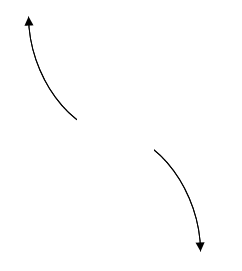
\includegraphics[width = 0.3\textwidth]{../Figures/polyEndBehaviorAB.png}\item 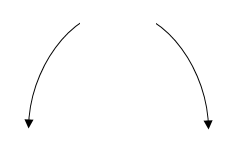
\includegraphics[width = 0.3\textwidth]{../Figures/polyEndBehaviorBB.png}\item 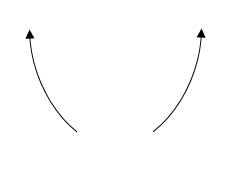
\includegraphics[width = 0.3\textwidth]{../Figures/polyEndBehaviorCB.png}\item 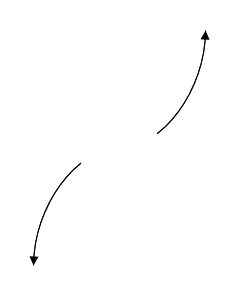
\includegraphics[width = 0.3\textwidth]{../Figures/polyEndBehaviorDB.png}\end{multicols}\item None of the above.
\end{enumerate} }
\litem{
Describe the end behavior of the polynomial below.\[ f(x) = 7(x - 4)^{4}(x + 4)^{5}(x + 3)^{3}(x - 3)^{5} \]\begin{enumerate}[label=\Alph*.]
\begin{multicols}{2}\item 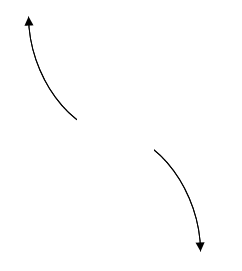
\includegraphics[width = 0.3\textwidth]{../Figures/polyEndBehaviorCopyAB.png}\item 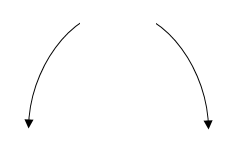
\includegraphics[width = 0.3\textwidth]{../Figures/polyEndBehaviorCopyBB.png}\item 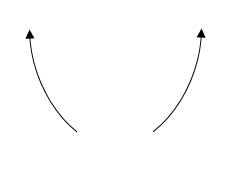
\includegraphics[width = 0.3\textwidth]{../Figures/polyEndBehaviorCopyCB.png}\item 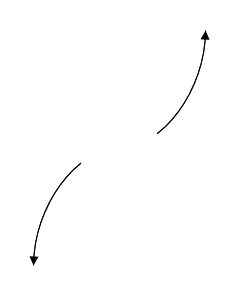
\includegraphics[width = 0.3\textwidth]{../Figures/polyEndBehaviorCopyDB.png}\end{multicols}\item None of the above.
\end{enumerate} }
\litem{
Construct the lowest-degree polynomial given the zeros below. Then, choose the intervals that contain the coefficients of the polynomial in the form $ax^3+bx^2+cx+d$.\[ 7, \frac{-1}{5}, \text{ and } \frac{2}{3} \]\begin{enumerate}[label=\Alph*.]
\item \( a \in [15, 17], b \in [110.6, 112.3], c \in [44, 57], \text{ and } d \in [-17, -12] \)
\item \( a \in [15, 17], b \in [91.8, 95.9], c \in [-92, -82], \text{ and } d \in [14, 19] \)
\item \( a \in [15, 17], b \in [-112.5, -108.4], c \in [44, 57], \text{ and } d \in [14, 19] \)
\item \( a \in [15, 17], b \in [96, 100.8], c \in [-52, -44], \text{ and } d \in [-17, -12] \)
\item \( a \in [15, 17], b \in [-112.5, -108.4], c \in [44, 57], \text{ and } d \in [-17, -12] \)

\end{enumerate} }
\litem{
Describe the zero behavior of the zero $x = 2$ of the polynomial below.\[ f(x) = -3(x + 2)^{4}(x - 2)^{5}(x - 7)^{5}(x + 7)^{7} \]\begin{enumerate}[label=\Alph*.]
\begin{multicols}{2}\item 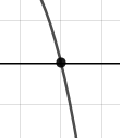
\includegraphics[width = 0.3\textwidth]{../Figures/polyZeroBehaviorAB.png}\item 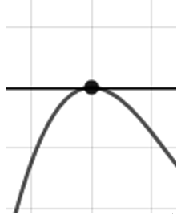
\includegraphics[width = 0.3\textwidth]{../Figures/polyZeroBehaviorBB.png}\item 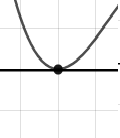
\includegraphics[width = 0.3\textwidth]{../Figures/polyZeroBehaviorCB.png}\item 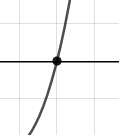
\includegraphics[width = 0.3\textwidth]{../Figures/polyZeroBehaviorDB.png}\end{multicols}\item None of the above.
\end{enumerate} }
\litem{
Which of the following equations \textit{could} be of the graph presented below?
\begin{center}
    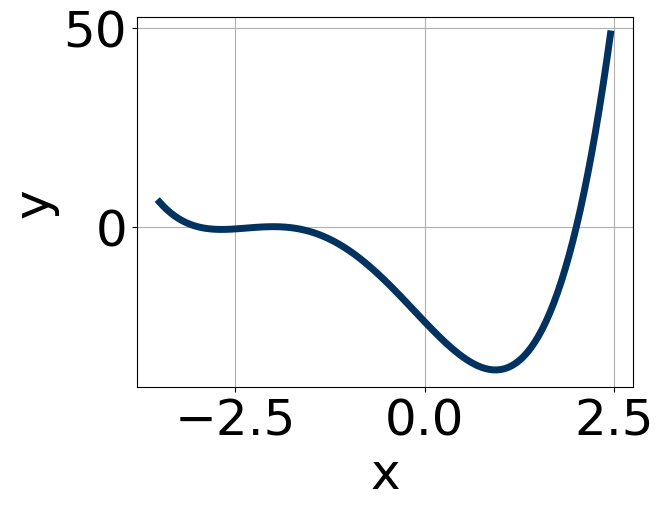
\includegraphics[width=0.5\textwidth]{../Figures/polyGraphToFunctionB.png}
\end{center}
\begin{enumerate}[label=\Alph*.]
\item \( -8(x - 2)^{10} (x + 4)^{6} (x + 1)^{5} \)
\item \( 12(x - 2)^{8} (x + 4)^{7} (x + 1)^{7} \)
\item \( -4(x - 2)^{10} (x + 4)^{11} (x + 1)^{11} \)
\item \( 11(x - 2)^{7} (x + 4)^{9} (x + 1)^{9} \)
\item \( -10(x - 2)^{5} (x + 4)^{7} (x + 1)^{11} \)

\end{enumerate} }
\litem{
Construct the lowest-degree polynomial given the zeros below. Then, choose the intervals that contain the coefficients of the polynomial in the form $x^3+bx^2+cx+d$.\[ 4 + 5 i \text{ and } 1 \]\begin{enumerate}[label=\Alph*.]
\item \( b \in [-11, -5], c \in [48.79, 49.11], \text{ and } d \in [-41.09, -39.64] \)
\item \( b \in [1, 6], c \in [-5.16, -3.28], \text{ and } d \in [2.13, 4.62] \)
\item \( b \in [1, 6], c \in [-6.36, -5.54], \text{ and } d \in [4.44, 5.18] \)
\item \( b \in [3, 14], c \in [48.79, 49.11], \text{ and } d \in [39.48, 43] \)
\item \( \text{None of the above.} \)

\end{enumerate} }
\litem{
Describe the zero behavior of the zero $x = -7$ of the polynomial below.\[ f(x) = -9(x - 4)^{5}(x + 4)^{2}(x + 7)^{11}(x - 7)^{8} \]\begin{enumerate}[label=\Alph*.]
\begin{multicols}{2}\item 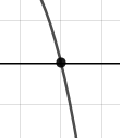
\includegraphics[width = 0.3\textwidth]{../Figures/polyZeroBehaviorCopyAB.png}\item 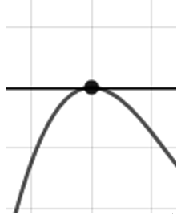
\includegraphics[width = 0.3\textwidth]{../Figures/polyZeroBehaviorCopyBB.png}\item 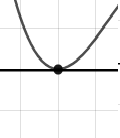
\includegraphics[width = 0.3\textwidth]{../Figures/polyZeroBehaviorCopyCB.png}\item 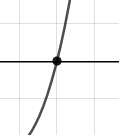
\includegraphics[width = 0.3\textwidth]{../Figures/polyZeroBehaviorCopyDB.png}\end{multicols}\item None of the above.
\end{enumerate} }
\litem{
Construct the lowest-degree polynomial given the zeros below. Then, choose the intervals that contain the coefficients of the polynomial in the form $ax^3+bx^2+cx+d$.\[ -1, \frac{-4}{5}, \text{ and } \frac{3}{5} \]\begin{enumerate}[label=\Alph*.]
\item \( a \in [19, 32], b \in [28, 33], c \in [-10, -3], \text{ and } d \in [12, 19] \)
\item \( a \in [19, 32], b \in [-26, -18], c \in [-20, -16], \text{ and } d \in [12, 19] \)
\item \( a \in [19, 32], b \in [-64, -56], c \in [45, 49], \text{ and } d \in [-12, -9] \)
\item \( a \in [19, 32], b \in [28, 33], c \in [-10, -3], \text{ and } d \in [-12, -9] \)
\item \( a \in [19, 32], b \in [-32, -26], c \in [-10, -3], \text{ and } d \in [12, 19] \)

\end{enumerate} }
\litem{
Which of the following equations \textit{could} be of the graph presented below?
\begin{center}
    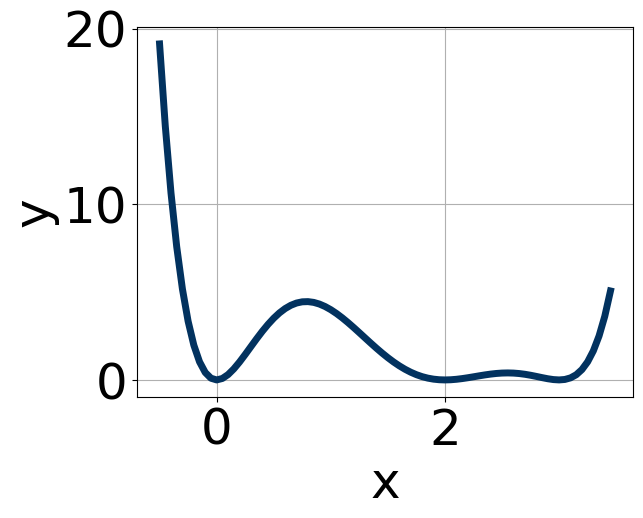
\includegraphics[width=0.5\textwidth]{../Figures/polyGraphToFunctionCopyB.png}
\end{center}
\begin{enumerate}[label=\Alph*.]
\item \( 12(x + 3)^{8} (x - 2)^{11} (x - 3)^{9} \)
\item \( -19(x + 3)^{6} (x - 2)^{10} (x - 3)^{11} \)
\item \( -20(x + 3)^{9} (x - 2)^{6} (x - 3)^{9} \)
\item \( 6(x + 3)^{4} (x - 2)^{11} (x - 3)^{4} \)
\item \( -5(x + 3)^{6} (x - 2)^{5} (x - 3)^{9} \)

\end{enumerate} }
\end{enumerate}

\end{document}